% !TeX spellcheck = it_IT
\documentclass[10pt]{article}
\usepackage{color, soul}
\newcommand{\hlc}[2][yellow]{ {\sethlcolor{#1} \hl{#2}} }
\usepackage[T1]{fontenc}
\usepackage{float}
\usepackage[utf8]{inputenc}
\usepackage[margin=1in]{geometry}
\usepackage{listings}
\usepackage{graphicx}
\usepackage[italian]{babel}
\usepackage[hidelinks]{hyperref}
\title{IMAGine}
\author{Francesco Paolo Castiglione, Davide Iraci, Andrea Montemaggiore}
\date{Settembre 2020}

\begin{document}
	\maketitle
	\tableofcontents
	\clearpage

\section{Introduzione}IMAGine (IMAge-enGINE) è un linguaggio ideato per l’elaborazione delle immagini a trecentosessanta gradi. Il linguaggio consente le elaborazioni più comuni attraverso un processo immediato ed intuitivo.
E’ stato pensato e sviluppato tenendo conto di alcuni fattori chiavi quali semplicità d’uso e rapidità di apprendimento, basandosi anche su altri linguaggi già esistenti quali MATLAB, Python o software per la modifica di immagini.\newline
Il resto della relazione è strutturato come segue: la sezione 2 illustra il contesto in cui si colloca il linguaggio proposto, nella sezione 3 vengono analizzati i dettagli implementativi, nella sezione 4 si illustrano le caratteristiche di IMAGine e degli esempi di applicazioni, infine nella sezione 5 vengono riepilogati i punti principali del lavoro svolto.
\clearpage
\section{Stato dell'arte}Attualmente l’Image Processing avviene principalmente per mezzo di software già pronti quali Photoshop, Gimp, etc. Questi software sono stati pensati per un utilizzo da parte di amanti delle immagini e per professionisti in campo fotografico. Alcuni di questi, come il già citato Adobe Photoshop vengono proposti in una suite software chiamata “Adobe Creative 2020”, la quale, nella sua ultima edizione, comprende altri applicativi per l’Image Processing di livello sempre più alto.
Per lo sviluppo del progetto ci siamo principalmente basati sullo stato dell’arte dei linguaggi che permettono operazioni su immagini e sulle operazioni che permettono: da semplici  rotazioni, zooming e shrinking alle più complicate operazioni di edge detection, cambio dello spazio di colori, etc;\newline
Come linguaggio da adoperare per produrre il progetto sono stati individuati linguaggi dalla sintassi concisa ed efficace quali C, C++, Java e Python. Ognuno di detti linguaggi ha pro e contro ma tutti richiedono l’utilizzo di librerie esterne per l’implementazione delle modifiche e operazioni su immagini. C e Python sono attualmente i più veloci. C presenta una sintassi più complessa per l’utilizzo delle relative librerie mentre Python possiede numerose librerie con una sintassi di facile utilizzo ma alcune di esse, o meglio quasi tutte, non ottengono un buon risultato performando alcune operazioni più complicate come edge detection. Va sottolineato come il package “skimage” per Python sia uno dei migliori in termini di prestazioni e risultati. Per C e C++ la libreria migliore in termini di prestazioni è “LibVips” adoperata anche in questo progetto, nonostante possieda una sintassi di difficile utilizzo per via dei lunghi nomi dei metodi. L’ultima analisi si basa su Matlab, ampiamente usato, specialmente in ambito accademico. Si tratta del linguaggio per immagini per eccellenza. Alcune operazioni, come media adattiva, mediano adattivo, etc, richiedono che il programmatore abbia una conoscenza approfondita del linguaggio ed ambiente di sviluppo MATLAB, mentre per operazioni più semplici, quale applicazione di filtri di media e mediano, è sufficiente utilizzare funzioni built-in.
Dallo stato dell’arte vengono dunque individuati i passaggi chiave per la creazione del linguaggio: sintassi semplici e prestazioni d’alto livello.
\clearpage
\section{Descrizione del progetto}In questa sezione vengono illustrate le scelte progettuali e le motivazioni che hanno portato alla scelta della libreria LibVips.\\
IMAGine, volendo emulare Python, ha un funzionamento da interprete interattivo, quindi lanciando l'eseguibile è possibile "programmare  live". E' viceversa possibile indicare come secondo argomento un file da mandare in pasto all'interprete il quale leggerà e valuterà man mano le espressioni inserite. E' stato creato un helper per aiutare gli utenti nell'utilizzo del linguaggio. Esso è utilizzabile dal terminale, richiamando l'eseguibile inserendo come secondo argomento la stringa \texttt{help}, o durante l'esecuzione con attraverso il comando \texttt{\#help?}.
\subsection{Scelte progettuali}
Dal punto di vista sintattico il team si è ispirato a linguaggi dalla sintassi intuitiva quali \textit{Javascript} , \textit{Python} e \textit{C\#}. Le variabili vengono dichiarate senza specificare un tipo esplicito. Il valore viene semplicemente assegnato alla variabile in fase di inizializzazione della stessa o successivamente. Le immagini vengono dichiarate fornendo il path, rendendo cosi' più manegevole l'elaborazione delle immagini. Il tipo ricorsivo lista può contenere qualunque elemento, compreso un tipo lista.\\
Particolare attenzione è stata prestata alla \textit{leggibilità} del codice IMAGine ed alla \textit{semplicità d'uso} nel dominio scelto, ovvero l'elaborazione delle immagini. Il linguaggio si presta all'utilizzo da parte di utenti occasionali e presenta una veloce curva di apprendimento.
\subsection{LibVips}
l team in fase di analisi ricercato al fine di individuare una libreria che fosse veloce e che allo stesso tempo non usasse una alta quantità di memoria per le operazioni effettuate sulle immagini. A tal proposito il team ha valutato i risultati dei benchmarks sulle librerie. Da tale analisi è apparso chiaro che LibVips si classivica per 0.04 secondi come seconda libreria più veloce utilizzando in media ben 100 mb di memoria in meno rispetto alla prima classificata per la stessa operazione. In figura \ref{fig:benchmark1} viene riportata una tabella contenente delle informazioni sui benchmarks risultato dell'operazione di copia di un' immagine di 5000x5000 pixel 8-bit RGB in formato TIFF non compressa.\\
Si può facilmente notare che LibVips lanciato in modalità one thread o in modalità command-line rimane comunque una delle librerie più affidabili. Inoltre nella lunga lista di alternative non sono presenti esclusivamente librerie di image processing per C/C++ ma anche librerie per Python come la famosa SciPy basata su NumPy. In figura \ref{fig:benchmark0} vengono riportati i relativi dati.\\
Analizzando meglio le varie implementazioni ci si è resi conto che VipLips in modalità command-line genera un grosso traffico di dati sul disco. In figura \ref{fig:benchmark2} è possibile notare come LibVips (ultimo nella legenda) sia quello che utilizza meno memoria e meno tempo e quindi la miglior libreria utilizzabile.\\
Un’altra serie di benchmarks, illustrati in figura \ref{fig:benchmark3}  è stata effettuata prendendo un’immagine di 10000x10000 pixel scattata da una macchina digitale sulla quale sono successivamente state applicate le seguenti operazioni : sottoposta a cambio di spazio di colori, ridimensionata, tagliata (cropping) e sottoposta ad operazione di sharpening. Tale operazione è stata effettuata su diversi processi, alcuni di livello server ad altri di uso domestico.\\
Si può notare che perfino su dispositivi completamente diversi come Raspberry Pi 2 il tempo per l’operazione non sia altissimo, considerando che  l’utilizzo di questa libreria rimane una delle poche opzioni a disposizione dell’utente in quanto sicuramente le suite di software con interfaccia grafica, ad esempio Adobe Creative, non possono essere utilizzate agevolmente su alcuni degli ultimi processori/dispositivi in figura \ref{fig:benchmark3} .\clearpage

\begin{figure}
	\centering
	\resizebox{\columnwidth}{!}{
		
\includegraphics{sources/bench0.png}}
	\caption{Risultato benchmark SciPy}
	\label{fig:benchmark0}
\end{figure}

\begin{figure}
	\centering
	\resizebox{\columnwidth}{!}{
		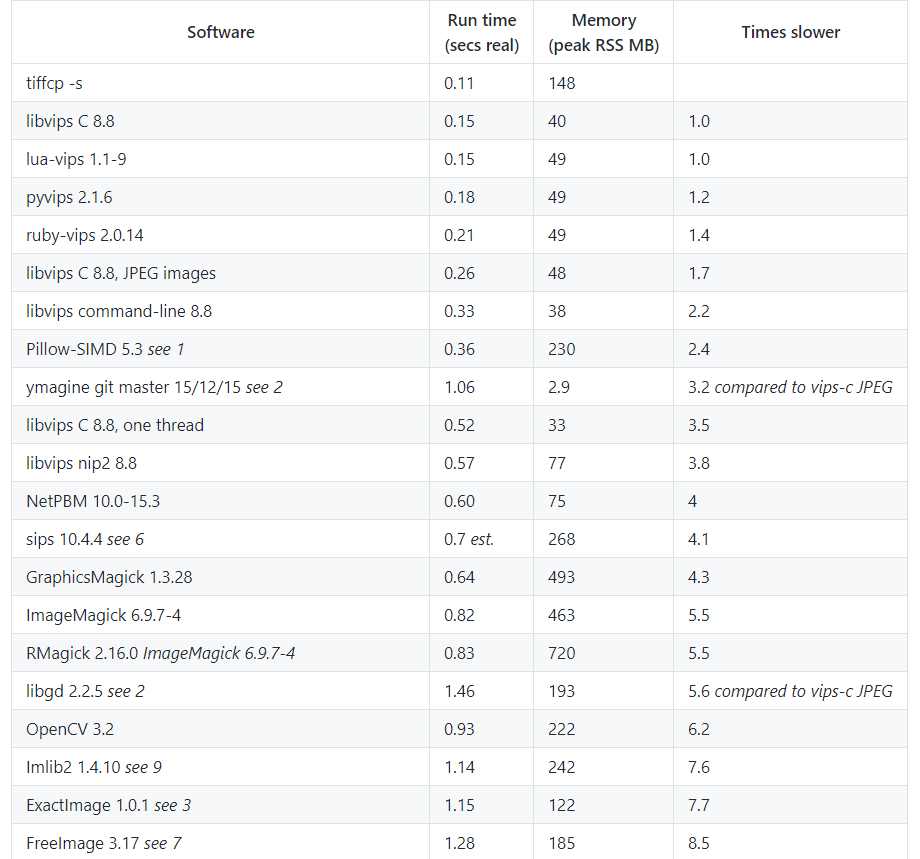
\includegraphics{sources/bench1.png}}
	\caption{Risultato benchmark}
	\label{fig:benchmark1}
\end{figure}

\begin{figure}
\centering
\resizebox{\columnwidth}{!}{
	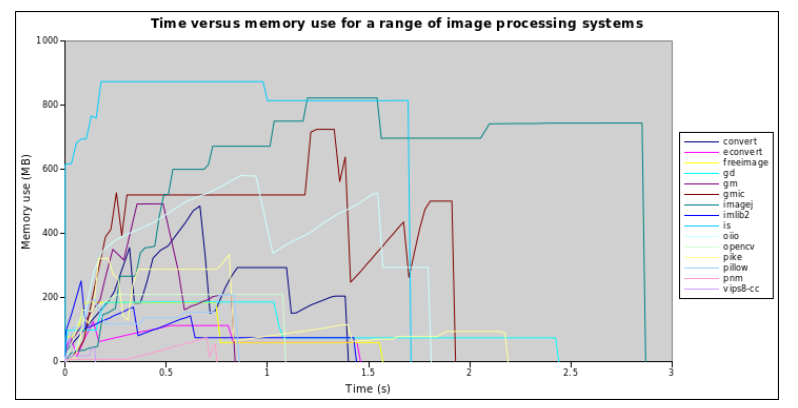
\includegraphics{sources/bench2.png}}
\caption{Risultato benchmark uso memoria}
\label{fig:benchmark2}
\end{figure}

\begin{figure}
	\centering
	\resizebox{12cm}{!}{
		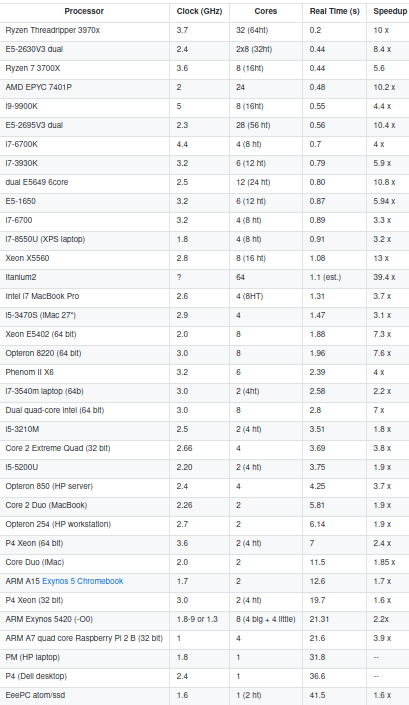
\includegraphics{sources/bench3.png}}
	\caption{Risultato benchmark}
	\label{fig:benchmark3}
\end{figure}

\clearpage
\subsection{Guida all'uso}
Per poter utilizzare il linguaggio in esame è necessario installare LibVips \cite{lipvips}, a tal proposito è consigliato scaricare il .tar dal seguente link : \url{https://github.com/libvips/libvips/releases}\\
Prima di installare la libreria è necessario installare le seguenti dependencies: \\
\texttt{build-essential, pkg-config, glib2.0-dev, libexpat1-dev, expat}
\\ Per ognuna di esse scrivere su terminale Unix \texttt{“sudo apt-get install XXX”}. Dopo aver fatto ciò si può installare Libvips tramite:\\\\
\texttt{tar xf vips-x.y.z.tar.gz}\\
\texttt{cd vips-x.y.z}\\
\texttt{./configure}\\\\
Sul terminale, dopo l’ultimo comando verranno specificate eventuali dependencies da installare. E' consigliato l'utilizzo del comando \texttt{sudo apt-get update}. Per concludere, quando il comando \texttt{./configure} non crea problemi:\\\\
\texttt{make}\\
\texttt{sudo make install}\\
\texttt{sudo ldconfig}\\
\clearpage
\section{Caratteristiche del linguaggio} 
\subsection{Grammatica}
\subsubsection{Tipi}
In seguito ad analisi relative ai possibili usi del linguaggio proposto, sono stati individuati i seguenti tipi primitivi:
\begin{itemize}
	\item \texttt{integer}, utilizzato per rappresentare i numeri interi
	\item \texttt{doublePrecision}, utilizzato per rappresentare i numeri in virgola mobile
	\item \texttt{str}, utilizzato per rappresentare le stringhe di caratteri
	\item \texttt{img}, utilizzato per rappresentare le immagini
\end{itemize}
E' stato inoltre individuato il tipo composto:
\begin{itemize}
	\item \texttt{list}, tipo ricorsivo
\end{itemize}
Le variabili di tipo \textit{int}, \textit{doublePrecision} e \textit{str} vengono dichiarate senza specificare un tipo esplicito.\\\\
\textit{\textbf{Esempio di dichiarazione ed assegnazione:}}\\\\
\textbf{stringVariable="this is a string";}\\
\textbf{intVariable=5;}\\
\textbf{doubleVariable=5.5;}\\
\textbf{img imageVariable="/path/img.png";}\\
\textbf{list li=\{1,2,"element"\};}\\

\subsubsection{Operazioni}
Il linguaggio consente le seguenti operazioni : somma, sottrazione, moltiplicazione, divisione, and e or logici, e paragoni ( ==, !=, >, >=, <, <=).

\begin{itemize}
	\item Il risultato di divisioni, prodotti, somme e differenze fra \textit{integer} e \textit{doublePrecision} è sempre un \textit{doublePrecision}.
	\item Il risultato di divisioni fra \textit{integer} è un \textit{doublePrecision}
	\item Il risultato di somme, prodotti e differenze fra tipi uguali mantiene il tipo degli elementi iniziali
\end{itemize}

\textbf{String1 == String2 valuta il contenuto delle stringhe}\\
\textbf{String1 != String2 valuta il contenuto delle stringhe}\\

Le combinazioni di tipi consentite per ogni operatore sono riassunte nella tabella~\ref{table:operatori}. I paragoni e gli operatori logici restituiscono sempre degli int, tutti gli altri operatori restituiscono un valore del tipo della colonna, tranne la moltiplicazione \texttt{int * string} equivalente a \texttt{string * int}. Le operazioni illustrate non sono ammesse per il tipo immagine e per il tipo lista.\\



\begin{table}
	\centering
	\begin{tabular}{|c|c|c|c|c|c|c|}
		\hline
		V1\textbackslash V2   &        int            &    double             &  string       \\ \hline
		int                    &  + - * / or and CMP   &  + - * / or and CMP   &    *          \\ \hline
		double       			& + - * / or and CMP    & + - / * CMP   		&     +         \\ \hline
		string        		     &        + *             &         +      	     & +    CMP      \\ \hline
	\end{tabular}
	\caption{Operazioni consentite dal linguaggio, sono da intendersi come V1 <operatore> V2. Con CMP si indicano le operazioni di comparazione}
	\label{table:operatori}
\end{table}
\newpage
\subsubsection{Strutture di controllo}
Il linguaggio fornisce la possibilità di usare sia comandi condizionali che comandi iterativi. I comandi condizionali sono i seguenti:
\begin{itemize}
	\item \texttt{if ( condition ) then \{ instructions \};}
	\item \texttt{if ( condition ) then \{ instructions \} else \{ instructions \}}
\end{itemize}
I comandi iterativi sono qui elencati :
\begin{itemize}
	\item \texttt{while ( condition ) do \{ instructions \}}
	\item \texttt{foreach ( tempElement : list ) \{ instructions \} }
\end{itemize}
Nell'espressione \texttt{while} si itera indefinitivamente finché la condizione non è più verificata. Nle costrutto \texttt{foreach} si itera invece per ogni elemento contenuto nella lista. E' possibile effettuare operazioni sull'elemento della lista tempElement, anche nel caso in cui si tratti di un'immagine. Questo rende possibile l'elaborazione di una lista di immagini.\\

\subsubsection{Funzioni}
Il linguaggio presenta una ricca selezione di funzioni built-in. All'utente viene inoltre fornita la possibilità di definire la propria funzione custom, con sintassi:\\\\ ``\texttt{def nome\_funzione ( parametri\_formali ) \{ istruzioni \}}''.
\clearpage
\subsection{Parser}
Il linguaggio è stato progettato con i tools Bison e Flex, due strumenti per costruire programmi che gestiscano input strutturati. Flex si occupa dell'analisi lessicale (lexing) mentre Bison si occupa dell'analisi sintattica (parsing). L'output dei due tools è un parser di tipo LALR(1) che effettua un parsing bottom-up, con cui è possibile gestire  produzioni left-recursive, utilizzando Bison per generare il parser e Flex per riconoscere i token nella fase di lexing.

Riportiamo di seguito le regole di produzione in formato BNF del linguaggio proposto:

\begin{lstlisting}
<program>::=
| HELP
| <program> <stmt>    
| <program> DEF NAME '(' <symlist> ')' '{' <list> '}' 
| <program> LIST NAME '=''{' elements '}' ';' 
| <program> error '\n'

<stmt>::= IF '(' <exp> ')' THEN '{' <list> '}' ';'                
| IF '(' <exp> ')' THEN '{' list '}' ELSE '{' <list> '}'   
| WHILE '('<exp> ')' DO '{' <list> '}'                    
| FOREACH '(' <foreach> ')' '{' <list> '}'                 
| exp ';'

<list>::=                               
| <stmt>  <list>                    

<exp>::= <exp> AND <exp>          
|<exp> OR <exp>           
| <exp> CMP <exp>          
| <exp> '+' <exp>          
| <exp> '-' <exp>       
| <exp> '*' <exp>        
| <exp> '/' <exp>       
| '|' <exp> '|'          
| '(' <exp> ')'          
| FUNC '(' <explist> ')' 
| NAME '=' <exp>         
| IMG NAME '=' <img>     
| NAME '(' <explist> ')' 
| <value>                

<foreach>::=    <name> ':' <name>        

<name>::= NAME                       

<value>::=  '-' INT %prec UMINUS      
| INT                          
| '-' DOUBLE %prec UMINUS      
| DOUBLE                       
| STRING                       
| NAME                         

<img>::=  STRING              
| FUNC '(' <explist> ')' 

<explist>::= <exp>          
| <exp> ',' <explist>  

<symlist>::= NAME         
| NAME ',' <symlist> 

<elements>::=                
| <value>               
| <value> ',' <elements>  

\end{lstlisting}

Si possono eliminare le ambiguità della grammatica attraverso strumenti che permettono di specificare la precedenza degli operatori eliminando le possibili ambiguità e scartando automaticamente gli alberi di parsing non validi, consentendo l'utilizzo di una grammatica più semplice e compatta. A tal proposito sono utilizzati gli operatori di precedenza %left %right.
\clearpage
\subsection{Lexer}
Nel lexer vengono adoperate delle regex per matchare i nomi delle variabili,le stringe,i numeri interi,i numeri in virgola mobile, l'inserimento di commenti, i simboli per i confronti, operazioni consentite sui tipi, i simboli consentiti, le funzioni built-in del linguaggio e le strutture di controllo. \\\\

\textbf{Help method}
\begin{lstlisting}[breaklines=true, postbreak=\mbox{{$\hookrightarrow$}\space}]
/* shows helper */
"#help?"             
\end{lstlisting}

\textbf{Valori}
\begin{lstlisting}[breaklines=true, postbreak=\mbox{{$\hookrightarrow$}\space}]
/* string */
\"{1}.[^"]*\"{1}      

/* int */
[0-9]+                

/* double */
[0-9]+\.{1}[0-9]+    
\end{lstlisting}

\textbf{Tipi espliciti}
\begin{lstlisting}[breaklines=true, postbreak=\mbox{{$\hookrightarrow$}\space}]
"img"   
"list" 
"def"   
\end{lstlisting}

\textbf{Nome variabili}
\begin{lstlisting}[breaklines=true, postbreak=\mbox{{$\hookrightarrow$}\space}]
/* names */
[a-zA-Z][a-zA-Z0-9]*  
\end{lstlisting}

\textbf{Simboli}
\begin{lstlisting}[breaklines=true, postbreak=\mbox{{$\hookrightarrow$}\space}]
"+" 
"-" 
"*" 
"/" 
"=" 
"|" 
"," 
";" 
"(" 
"{" 
"}" 
":" 
")"     
\end{lstlisting}

\textbf{Paragoni}
\begin{lstlisting}[breaklines=true, postbreak=\mbox{{$\hookrightarrow$}\space}]
">"     
"<"    
"!="    
"=="   
">="    
"<="    
\end{lstlisting}
\clearpage
\textbf{Operatori logici}
\begin{lstlisting}[breaklines=true, postbreak=\mbox{{$\hookrightarrow$}\space}] 
"&&"    
"||"   
\end{lstlisting}

\textbf{Strutture di controllo ed iterative}
\begin{lstlisting}[breaklines=true, postbreak=\mbox{{$\hookrightarrow$}\space}]
 "if"   
 "then"  
 "else" 
 "while" 
 "do"    
 "foreach" 
\end{lstlisting}

\textbf{Funzioni built-in}
\begin{lstlisting}[breaklines=true, postbreak=\mbox{{$\hookrightarrow$}\space}]
"print"     
\end{lstlisting}

\textbf{Funzioni built-in per elaborazione immagini}
\begin{lstlisting}[breaklines=true, postbreak=\mbox{{$\hookrightarrow$}\space}]
"width"             
"height"            
"bands"             
"min"               
"max"               
"average"           
"invert"            
"histEq"            
"normalise"         
"canny"             
"sobel"             
"sharpen"          
"convert"           
"convertColorSpace" 
"add"               
"subtract"        
"rotate"           
"flip"          
"gaussianBlur"    
"smartCrop"        
"zoom"             
"crop"             
"showImage"               
\end{lstlisting}


\textbf{Funzioni built-in per liste}
\begin{lstlisting}[breaklines=true, postbreak=\mbox{{$\hookrightarrow$}\space}]
"length"           
"push"             
"insert"           
"remove"            
"pop"               
"get"               
\end{lstlisting}

\textbf{Commenti}
\begin{lstlisting}[breaklines=true, postbreak=\mbox{{$\hookrightarrow$}\space}]
"//".*  
[ \t]   /* ignore white space */ 
\\\n    /* ignore line continuation */
"\n"  
\end{lstlisting}

\subsection{Funzionalità del linguaggio}
\subsubsection{Metodo print}
Il metodo \textbf{print(var)} stampa su terminale il contenuto di \textbf{var}. Accetta qualunque tipo come argomento. 
\textbf{In generale}, \textit{print(var + string)} stamperà su schermo la concatenazione delle due variabili, indipendentemente dal tipo di \textit{var} (che verrà convertita a stringa).\\ 
E' anche possibile ripetere una stringa \textbf{n} volte utilizzando all'interno del metodo l'operatore \textbf{*}\\\\
\textbf{print(3*string) stamperà per tre volte il contenuto di string}\\
\textbf{print(3+string) stamperà la concatenazione fra la 3 e il contenuto di string}\\
\textbf{print(string1+string2) stamperà la concatenazione fra le due stringhe}\\

\subsubsection{Metodi per le liste}
Vengono qui elencati i metodi per le liste. \textit{Element} può essere un tipo qualunque, perfino una lista, in quanto le liste di liste sono permesse.\\

\begin{itemize}
\item \texttt{int length(list list\_name)} restituisce la lunghezza della lista ;
\item \texttt{void push(list list\_name, element)} inserisce un elemento nella lista(all'ultimo posto) ;
\item \texttt{void insert(list list\_name, element, int position)} inserisce un elemento nella posizione desiderata ;
\item \texttt{void remove(list list\_name, int position);} rimuove l’elemento dalla posizione desiderata ;
\item \texttt{element pop(list list\_name)} rimuove e restituisce l’ultimo elemento ;	
\item \texttt{element get(list list\_name, int position)} restituisce l‘elemento nella posizione desiderata ;
\end{itemize}

\subsubsection{Metodi per le immagini}
Di seguito vi sono tutte le operazioni delle immagini con una breve descrizione delle loro operazioni.\\


\begin{itemize}
\item \texttt{int width(img name\_image)} restituisce la larghezza dell’immagine in pixel ;
\item \texttt{int height(img name\_image)} restituisce l'altezza dell’immagine in pixel ;
\item \texttt{int bands(img name\_image)} restituisce il numero di canali presenti nell’immagine ;
\item \texttt{double min(img name\_image)} restituisce il minimo valore dei pixel nell’immagine ;
\item \texttt{double max(img name\_image)} restituisce il massimo valore dei pixel dell’immagine ;	
\item \texttt{double average(img name\_image)} restituisce il valore medio dei pixel dell’immagine ;
\item \texttt{img invert(img name\_image, char* output\_path)} restituisce e salva l'immagine invertita ;
\item \texttt{img histEq (img name\_image, char* output\_path)} restituisce e salva un’immagine sottoposta a equalizzazione dell’istogramma ;
\item \texttt{img normalise(img name\_image, char* output\_path)} restituisce e salva un’immagine sottoposta a normalizzazione ;
\item \texttt{img canny(img name\_image, char* output\_path)} individua gli edge con il metodo di Canny, salva e restituisce l’immagine ;
\item \texttt{img sobel(img name\_image, char* output\_path)} individua gli edge con il metodo di Sobel, salva e restituisce l’immagine ;
\item \texttt{img sharpen(img name\_image, char* output\_path)} esegue un blur gaussiano e lo sottrae all’immagine originale per generare un segnale d’alta frequenza. Ritorna e salva l’immagine risultante ;
\item \texttt{img convert(img name\_image, char* output\_path)} ritorna e salva l’immagine con un output specifico* ;
\item \texttt{img convertColorSpace(img name\_image, char* output\_path, char* space)} sposta l'immagine nello spazio dei colori indicato, salva e restituisce l’immagine** ;
\item \texttt{img add (img name\_image, img name\_image2, char* output\_path)} restituisce e salva la somma bit a bit di due immagini ;
\item \texttt{img subtract (img name\_image, img name\_image2, char* output\_path)} restituisce e salva la differenza bit a bit di due immagini ;
\item \texttt{img rotate(img name\_image, char* output\_path, double rotate\_angle)} restituisce e salva l’immagine di input rotata di un certo angolo ;
\item \texttt{img flip(img name\_image, char* output\_path, char* direction)} restituisce e salva l’immagine di input capovolta in una certa direzione (verticale/orizzontale) ;
\item \texttt{img gaussianBlur(img name\_image, char* output\_path, double mask\_dim)} restituisce e salva l’immagine di input sottoposta a blur gaussiano con maschera di dimensioni specificate in input ;
\item \texttt{img smartCrop (img name\_image, char* output\_path, double width, double height)} ritaglia un’immagine,la salva e la restituisce. La selezione delle parti da ritagliare avviene con un algoritmo che cerca di individuare le caratteristiche di maggiore interesse per gli esseri umani ;
\item \texttt{img zoom(img name\_image, char* output\_path, int xfactor, int yfactor)} restituisce e salva l’immagine ingrandita in base a due fattori di zoom x e y ;
\item \texttt{img crop(img name\_image, char* output\_path, double left, double top, double width, double height)} itaglia un’immagine,la salva e la restituisce. Le dimensioni della porzione da ritagliare sono fornite in input (rispettivamente distanza in pixel dal margine sinistro,distanza in pixel dal margine in alto, larghezza ed altezza);
\end{itemize}

*Formati ammessi:
\begin{itemize}
	\item tif
	\item jpeg or jpg
	\item hdr
	\item raw
	\label{itm:formats}
\end{itemize}

**Spazi dei colori ammessi:
\begin{itemize}
	\item grey16
	\item hsv
	\item yxy
	\item lch
	\item cmc
	\item lab
\end{itemize}
\clearpage
\section{Casi d'uso}




\subsection{Primo caso}
\lstinputlisting[firstline=1, lastline=62, frame=single, numbers=left, stepnumber=1, captionpos=b, caption={Sorgente firstCase.ig}, label={listing:sub}, breaklines=true, postbreak=\mbox{{$\hookrightarrow$}\space}
]{../program/UseCases/firstCase.ig}
\clearpage


\subsection{Secondo caso}
\lstinputlisting[firstline=1, lastline=62, frame=single, numbers=left, stepnumber=1, captionpos=b, caption={Sorgente secondCase.ig}, label={listing:sub}, breaklines=true, postbreak=\mbox{{$\hookrightarrow$}\space}
]{../program/UseCases/secondCase.ig}
\clearpage


\subsection{Terzo caso}
\lstinputlisting[firstline=1, lastline=62, frame=single, numbers=left, stepnumber=1, captionpos=b, caption={Sorgente thirdCase.ig}, label={listing:sub}, breaklines=true, postbreak=\mbox{{$\hookrightarrow$}\space}
]{../program/UseCases/thirdCase.ig}

\clearpage
\section{Risultati}
Al fine di testare la performance di IMAGine sono stati effettuati dei test su alcuni fra i più noti problemi calcolo quali il fattoriale e il pi greco. Infine viene effettuato un paragone con MATLAB al fine di testare operazioni nel dominio applicativo del linguaggio, ovvero l'elaborazione delle immagini.

\subsection{Fattoriale}

\lstinputlisting[firstline=1, lastline=62, frame=single, numbers=left, stepnumber=1, captionpos=b, caption={Sorgente factorial.ig}, label={listing:sub}, breaklines=true, postbreak=\mbox{{$\hookrightarrow$}\space}
]{../program/Benchmark/factorial.ig}

\lstinputlisting[firstline=1, lastline=62, frame=single, numbers=left, stepnumber=1, captionpos=b, caption={Sorgente factorial.py}, label={listing:sub}, breaklines=true, postbreak=\mbox{{$\hookrightarrow$}\space}
]{../program/Benchmark/factorial.py}

\begin{figure}[H]
	\centering
	\resizebox{6cm}{!}{
		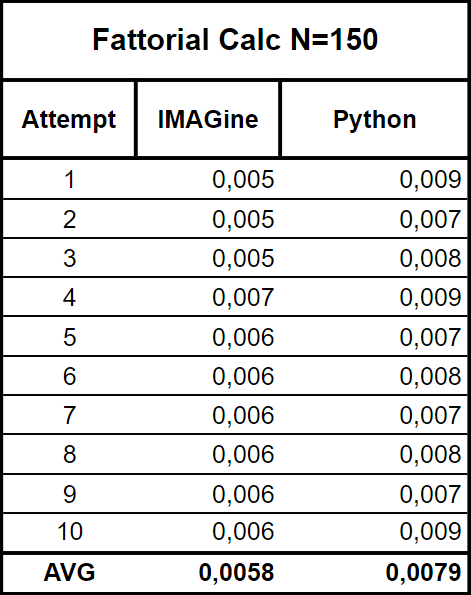
\includegraphics{sources/bench5-Fact.png}}
	\caption{Risultato benchmark}
	\label{fig:benchmarkFact2}
\end{figure}

\begin{figure}[H]
	\centering
	\resizebox{\columnwidth}{!}{
		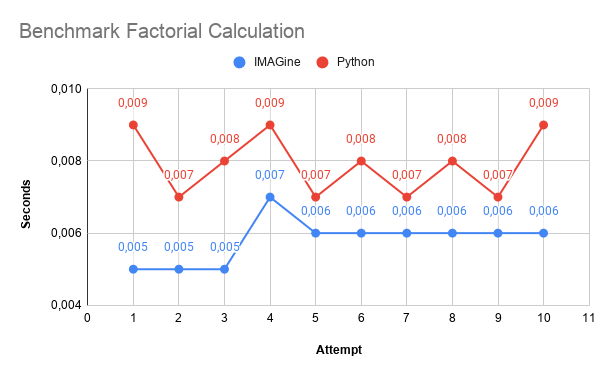
\includegraphics{sources/bench4-Fact.png}}
	\caption{Risultato benchmark}
	\label{fig:benchmarkFact1}
\end{figure}
\clearpage
\subsection{Pi greco}

\lstinputlisting[firstline=1, lastline=62, frame=single, numbers=left, stepnumber=1, captionpos=b, caption={Sorgente pigreco.ig}, label={listing:sub}, breaklines=true, postbreak=\mbox{{$\hookrightarrow$}\space}
]{../program/Benchmark/pigreco.ig}

\lstinputlisting[firstline=1, lastline=62, frame=single, numbers=left, stepnumber=1, captionpos=b, caption={Sorgente pigreco.py}, label={listing:sub}, breaklines=true, postbreak=\mbox{{$\hookrightarrow$}\space}
]{../program/Benchmark/pigreco.py}

\begin{figure}[H]
	\centering
	\resizebox{6cm}{!}{
		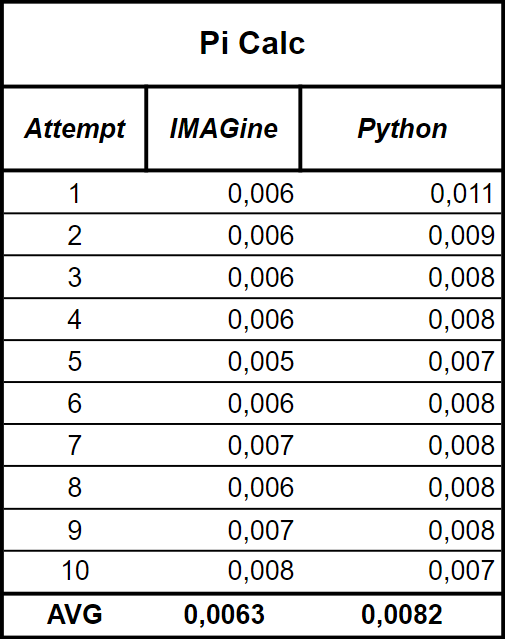
\includegraphics{sources/bench7-Pi.png}}
	\caption{Risultato benchmark}
	\label{fig:benchmarkFact2}
\end{figure}

\begin{figure}[H]
	\centering
	\resizebox{\columnwidth}{!}{
		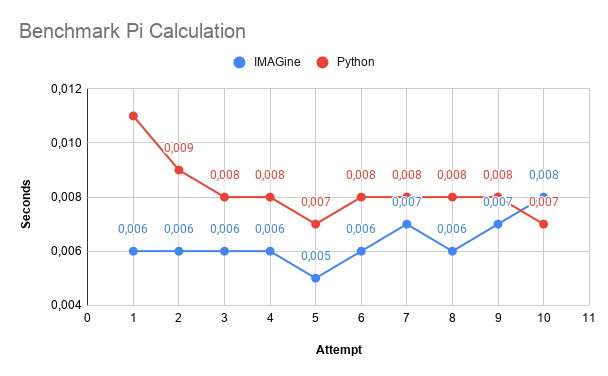
\includegraphics{sources/bench6-Pi.png}}
	\caption{Risultato benchmark}
	\label{fig:benchmarkFact1}
\end{figure}

\clearpage

\subsection{Restauro}

\lstinputlisting[firstline=1, lastline=62, frame=single, numbers=left, stepnumber=1, captionpos=b, caption={Sorgente gaussianrestore.ig}, label={listing:sub}, breaklines=true, postbreak=\mbox{{$\hookrightarrow$}\space}
]{../program/Benchmark/gaussianrestore.ig}

\lstinputlisting[firstline=1, lastline=62, frame=single, numbers=left, stepnumber=1, captionpos=b, caption={Sorgente gaussianrestore.m}, label={listing:sub}, breaklines=true, postbreak=\mbox{{$\hookrightarrow$}\space}
]{../program/Benchmark/gaussianrestore.m}

\begin{figure}[H]
	\centering
	\resizebox{6cm}{!}{
		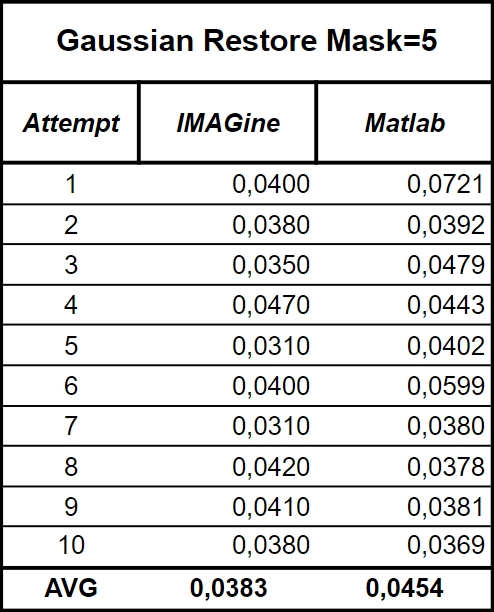
\includegraphics{sources/bench8-Gaussian.png}}
	\caption{Risultato benchmark}
	\label{fig:benchmarkFact2}
\end{figure}

\begin{figure}[H]
	\centering
	\resizebox{\columnwidth}{!}{
		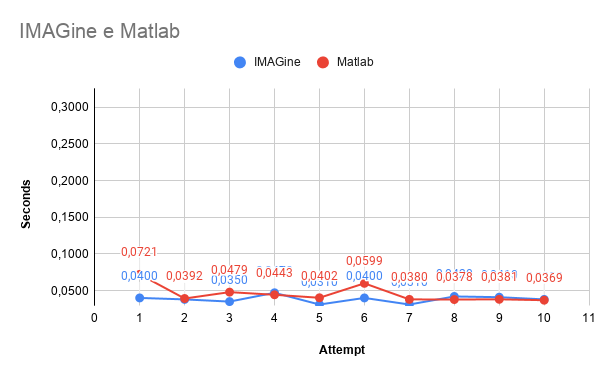
\includegraphics{sources/bench9-Gaussian.png}}
	\caption{Risultato benchmark}
	\label{fig:benchmarkFact1}
\end{figure}

\section{Conclusioni}
Durante lo sviluppo del linguaggio sono state affrontate numerose tematiche trattate durante il corso di \textit{Linguaggi e traduttori} . L'esperienza di sviluppo ha permesso al team di apprezzare l'importanza di solide fondamenta teoriche unite a una significativa esperienza pratica. Nonostante le tempistiche, le funzionalità ottenute risultano soddisfacenti .
\clearpage

%% BIBLIOGRAFIA
\clearpage
\bibliographystyle{unsrt}
\bibliography{tesina}
\begin{thebibliography}{toc}
	
	\bibitem[1]{lipvips}Libvips API documentation{ {\url{http://web.archive.org/web/20080207010024/http://www.808multimedia.com/winnt/kernel.htm}}}

	\bibitem[2]{book} John Levine.\textit{ Flex \& Bison: Text Processing Tools}. " O’Reilly Media, Inc.", 2009
\end{thebibliography}

\clearpage
\section*{Appendice}\label{section:appendix}
\addcontentsline{toc}{section}{Appendice}

\begin{center}
	\centering
	\resizebox{\columnwidth}{!}{
		\includegraphics{sources/parser.pdf}}\\
	Grafico del FSA generato utilizzando GNU Bison 3.5.4 XML Automaton Report. L'immagine è in formato vettoriale, quindi è possibile ingrandire a piacere.
\end{center}
\clearpage

\end{document}